\documentclass{scrartcl}
\usepackage[T1]{fontenc}
\usepackage{amsmath,amssymb}
\usepackage{newtxtext,newtxmath}
\usepackage[scale=0.85]{tgcursor}
\usepackage{microtype}
\usepackage{babel}
\usepackage{graphicx}
\usepackage{hyperref}


\title{Phong Shading with \LaTeX}
\author{Alan Xiang}
\date{\today}


\begin{document}

\maketitle

\ExplSyntaxOn


\newcommand{\DeclareConstFP}[2]
{
    \fp_if_exist:cF {#1}
    {
        \fp_new:c {#1}
    }
    \fp_gset:cn {#1} {#2}
}

\newcommand{\DeclareConstI}[2]
{
    \tl_if_exist:cF {#1}
    {
        \tl_new:c {#1}
    }
    \tl_gset:cn {#1} {#2}
}

% create a new binary output file
\tl_new:N \g_bin_filename_tl
\cs_new:Npn \bin_open:n #1
{
    \tl_gset:Nn \g_bin_filename_tl {#1}
    \iow_open:Nn \g_tmpa_iow {\jobname-bin.tmp}
}

\cs_new:Npn \bin_close:
{
    \iow_term:n {Converting~LaTeX~output~to~binary}
    \iow_close:N \g_tmpa_iow
    \exp_args:Nx \sys_shell_now:n {python3 ~ latex_output_to_binary.py ~ \jobname-bin.tmp ~ \g_bin_filename_tl}
}


% #1: value
\cs_new:Npn \bin_write_byte:n #1
{
    \iow_now:Nn \g_tmpa_iow {#1}
}


% #1: values
\cs_new:Npn \bin_write_byte_clist:n #1
{
    \clist_map_inline:nn {#1}
    {
        \bin_write_byte:n {##1}
    }
}


% writing (unsigned) binary value in small endian
% #1: value
% #2: number of bins
\int_new:N \l_bin_tmpa_int
\int_new:N \l_bin_tmpb_int
\cs_new:Npn \bin_write_bytes_se:nn #1#2
{
    \int_set:Nn \l_bin_tmpa_int {#1}
    \int_step_inline:nn {#2}
    {
        % get current byte
        \int_set:Nn \l_bin_tmpb_int {\int_mod:nn {\l_bin_tmpa_int} {256}}
        % proceed to next byte
        \int_set:Nn \l_bin_tmpa_int {\int_div_truncate:nn {\l_bin_tmpa_int} {256}}
        % write output
        \exp_args:Nx \bin_write_byte:n {\int_use:N \l_bin_tmpb_int}
    }
}

\cs_generate_variant:Nn \bin_write_bytes_se:nn {xn,xx}

% #1: width
% #2: height
\int_new:N \l_bin_tmpc_int
\cs_set:Npn \bin_write_bmp_header:nn #1#2
{
    % BMP file header

    \bin_write_byte:n {66} % B
    \bin_write_byte:n {77} % M
    
    % compute and write file size
    \int_set:Nn \l_bin_tmpc_int {54 + 3 * (#1) * (#2)}
    \bin_write_bytes_se:xn {\int_use:N \l_bin_tmpc_int} {4}

    \bin_write_byte_clist:n {0,0,0,0,54,0,0,0}

    % BMP info header
    \bin_write_byte_clist:n {40,0,0,0}
    \bin_write_bytes_se:xn {#1} {4} % width
    \bin_write_bytes_se:xn {#2} {4} % height
    \bin_write_byte_clist:n {1,0,24,0} % bytes per pixel
    \int_step_inline:nn {24}
    {
        \bin_write_byte:n {0}
    }
}

% these only exist in latest version
% \fp_set_function:nnn { norm } { a,b,c } { sqrt(a*a+b*b+c*c) }
% \fp_set_function:nnn { normalize } { a,b,c } { (a,b,c)/norm(a,b,c) }


\fp_new:N \l_myfp_tmph_fp
\fp_new:N \l_myfp_tmpi_fp
\tl_new:N \l_myfp_tmpb_tl
\tl_new:N \l_myfp_tmpc_tl
\tl_new:N \l_myfp_tmpd_tl
\tl_new:N \l_myfp_tmpe_tl
\tl_new:N \l_myfp_tmpf_tl
% element wise product
\cs_new:Npn \fp_prod:Nnn #1#2#3
{
    \tl_set:Nx \l_myfp_tmpb_tl {\fp_to_tl:n {#2}}
    \tl_set:Nx \l_myfp_tmpc_tl {\fp_to_tl:n {#3}}
    \tl_remove_all:Nn \l_myfp_tmpb_tl {(}
    \tl_remove_all:Nn \l_myfp_tmpb_tl {)}
    \tl_remove_all:Nn \l_myfp_tmpc_tl {(}
    \tl_remove_all:Nn \l_myfp_tmpc_tl {)}

    \tl_clear:N \l_myfp_tmpd_tl
    
    \bool_until_do:nn {\clist_if_empty_p:N \l_myfp_tmpb_tl}
    {
        \clist_pop:NN \l_myfp_tmpb_tl \l_myfp_tmpe_tl
        \clist_pop:NN \l_myfp_tmpc_tl \l_myfp_tmpf_tl
        \clist_put_right:Nx \l_myfp_tmpd_tl {\fp_eval:n {\l_myfp_tmpe_tl * \l_myfp_tmpf_tl}}
    }
    \fp_set:Nn #1 {(\l_myfp_tmpd_tl)}
}

% #1: compute dot product
\fp_new:N \l_myfp_tmpa_fp
\fp_new:N \l_myfp_tmpc_fp
\cs_new:Npn \fp_dot:Nnn #1#2#3
{
    \fp_prod:Nnn \l_myfp_tmpa_fp {#2} {#3}
    \fp_reduce_sum:Nn \l_myfp_tmpc_fp {\l_myfp_tmpa_fp}
    \fp_set_eq:NN #1 \l_myfp_tmpc_fp
}

\fp_new:N \l_myfp_tmpd_fp
\fp_new:N \l_myfp_tmpe_fp
\cs_new:Npn \fp_norm:Nn #1#2
{
    \fp_dot:Nnn \l_myfp_tmpd_fp {#2} {#2}
    \fp_reduce_sum:Nn \l_myfp_tmpe_fp {\l_myfp_tmpd_fp}
    \fp_set:Nn #1 {sqrt(\l_myfp_tmpe_fp)}
}

\fp_new:N \l_myfp_tmpf_fp
\fp_new:N \l_myfp_tmpg_fp
\cs_new:Npn \fp_normalize:Nn #1#2
{
    \fp_norm:Nn \l_myfp_tmpf_fp {#2}
    \fp_set:Nn #1 {#2 / \l_myfp_tmpf_fp}
}

\fp_new:N \l_myfp_tmpb_fp
\tl_new:N \l_myfp_tmpa_tl
\cs_new:Npn \fp_reduce_sum:Nn #1#2
{
    \tl_set:Nx \l_myfp_tmpa_tl {\fp_to_tl:n {#2}}
    \tl_remove_all:Nn \l_myfp_tmpa_tl {(}
    \tl_remove_all:Nn \l_myfp_tmpa_tl {)}
    \fp_set:Nn \l_myfp_tmpb_fp {0}
    \clist_map_inline:Nn \l_myfp_tmpa_tl
    {
        \fp_add:Nn \l_myfp_tmpb_fp {##1}
    }
    \fp_set_eq:NN #1 \l_myfp_tmpb_fp
}

\fp_new:N \l_myfp_tmpj_fp
\tl_new:N \l_myfp_tmpg_tl
\cs_new:Npn \fp_pixel_standardize:Nn #1#2
{
    \tl_set:Nx \l_myfp_tmpg_tl {\fp_to_tl:n {#2}}
    \tl_remove_all:Nn \l_myfp_tmpg_tl {(}
    \tl_remove_all:Nn \l_myfp_tmpg_tl {)}
    \tl_clear:N #1
    \clist_map_inline:Nn \l_myfp_tmpg_tl
    {
        \fp_set:Nn \l_myfp_tmpj_fp {max(min(##1,1.0),0.0)}
        \fp_set:Nn \l_myfp_tmpj_fp {round(255 * \l_myfp_tmpj_fp)}
        \clist_put_right:Nx #1 {\fp_to_int:N \l_myfp_tmpj_fp}
    }
}


\tl_new:N \l_bmp_row_tl
\tl_new:N \l_bmp_col_tl
\int_new:N \l_bmp_tmpa_int
\fp_new:N \l_bmp_tmpa_fp
\fp_new:N \l_bmp_tmpb_fp
\fp_new:N \l_bmp_tmpc_fp
\fp_new:N \l_bmp_tmpd_fp
\fp_new:N \l_bmp_norm_fp
\fp_new:N \l_bmp_view_fp
\fp_new:N \l_bmp_minhw_fp
\fp_new:N \l_bmp_x_fp
\fp_new:N \l_bmp_y_fp
\fp_new:N \l_bmp_z_fp
\fp_new:N \l_bmp_surface_fp
\fp_new:N \l_bmp_vdir_fp
\fp_new:N \l_bmp_ldir_fp
\fp_new:N \l_bmp_ndir_fp
\fp_new:N \l_bmp_rdir_fp
\fp_new:N \l_bmp_intensity_fp
\tl_new:N \l_bmp_tmpa_tl
\newcommand{\RenderToBMP}[1]
{
    % we do not want to deal with padding (lazy), so just make sure width is mulitple of 4
    \int_compare:nF {\int_mod:nn {\ImageWidth} {4} = 0}
    {
        \GenericError{}{BMP~width~must~be~multiple~of~4}{}{}
    }

    \bin_open:n {#1}
    
    % write BMP header
    \bin_write_bmp_header:nn {\ImageWidth} {\ImageHeight}

    \fp_set:Nn \l_bmp_minhw_fp {min(\ImageWidth,\ImageHeight)}

    % write BMP data
    \int_step_variable:nNn {\ImageHeight} \l_bmp_row_tl 
    {
        \iow_term:x {Rendering~BMP~line~\l_bmp_row_tl}
        \int_step_variable:nNn {\ImageWidth} \l_bmp_col_tl 
        {


            % assume orhographic camera

            % convert to relative pixel coordinate
            \fp_set:Nn \l_bmp_x_fp { ( \l_bmp_col_tl - (\l_bmp_minhw_fp)/2 ) / \l_bmp_minhw_fp}
            \fp_set:Nn \l_bmp_y_fp { ( \l_bmp_row_tl - (\l_bmp_minhw_fp)/2 ) / \l_bmp_minhw_fp}

            \fp_set:Nn \l_bmp_tmpa_fp { \l_bmp_x_fp ** 2 + \l_bmp_y_fp ** 2 }
            
            % insensity computation
            \fp_set:Nn \l_bmp_intensity_fp {(0,0,0)}

            \fp_compare:nT {\l_bmp_tmpa_fp <= 0.25}
            {
                % compute object surface location
                \fp_set:Nn \l_bmp_z_fp { sqrt( 0.25 - \l_bmp_tmpa_fp ) }

                % compute directions
                \fp_set:Nn \l_bmp_vdir_fp { (\l_bmp_x_fp, \l_bmp_y_fp, 1.0)  } % view directiion
                \fp_set:Nn \l_bmp_ldir_fp { \LightPos - (\l_bmp_x_fp, \l_bmp_y_fp, \l_bmp_z_fp)  } % light direction
                \fp_set:Nn \l_bmp_ndir_fp {(\l_bmp_x_fp, \l_bmp_y_fp, \l_bmp_z_fp)} % surface normal



                \fp_normalize:Nn \l_bmp_vdir_fp {\l_bmp_vdir_fp}
                \fp_normalize:Nn \l_bmp_ldir_fp {\l_bmp_ldir_fp}
                \fp_normalize:Nn \l_bmp_ndir_fp {\l_bmp_ndir_fp}

                

                \fp_dot:Nnn \l_bmp_tmpb_fp { \l_bmp_ldir_fp } { \l_bmp_ndir_fp }
                \fp_compare:nT { \l_bmp_tmpb_fp > 0} % visibility test
                {
                    \fp_set:Nn \l_bmp_rdir_fp { 2 * \l_bmp_tmpb_fp * \l_bmp_ndir_fp - \l_bmp_ldir_fp  } % reflection direction
    
                    \fp_add:Nn \l_bmp_intensity_fp {\kDiff * \l_bmp_tmpb_fp * \ObjectColor}
    
                    \fp_dot:Nnn \l_bmp_tmpc_fp { \l_bmp_rdir_fp } { \l_bmp_vdir_fp }
                    \fp_add:Nn \l_bmp_intensity_fp {\kSpec * (\l_bmp_tmpc_fp ** \kAlpha) * \SpecColor}
                }


                \fp_add:Nn \l_bmp_intensity_fp {\AmbientColor} % add ambient color
            }

            \fp_pixel_standardize:Nn \l_bmp_tmpa_tl {\l_bmp_intensity_fp}
            \clist_reverse:N \l_bmp_tmpa_tl % RGB to BGR
            \exp_args:NV \bin_write_byte_clist:n \l_bmp_tmpa_tl

        }
    }

    \bin_close:
}

\tl_new:N \l_time_now_tl
\cs_new:Npn \GetTime #1 
{
    \exp_args:Nx \sys_get_shell:nnN {date ~ +\c_percent_str s\c_percent_str 3N} {} \l_time_now_tl
    \tl_set:Nx #1 {\fp_eval:n {\l_time_now_tl / 1000.0}}
}

\cs_new:Npn \GetDuration #1#2
{
    \fp_eval:n {#2 - #1}
}

\newcommand{\ImgConv}[2]
{
    \iow_term:n {Converting~image~format...}
    \sys_shell_now:n {python3 ~ bmp_to_png.py ~ #1 ~ #2}
}

\newcommand{\RenderStat}{
    \par Rendering~configuration:

    \par \{
    \par \indent
    \begin{tabular}{lcl}
        height & = & \ImageHeight\\
        width & = & \ImageWidth \\
        kSpec & = & \fp_use:N \kSpec \\
        kDiff & = & \fp_use:N \kDiff \\
        kAlpha & = & \fp_use:N \kAlpha \\
        AmbientColor & = & \fp_use:N \AmbientColor \\
        ObjectColor & = & \fp_use:N \ObjectColor \\
        SpecColor & = & \fp_use:N \SpecColor \\
        LightPos & = & \fp_use:N \LightPos \\
        EyePos & = & \fp_use:N \EyePos
    \end{tabular}
    \par \}
}

\ExplSyntaxOff



\section*{Attempt 1}

{
\ttfamily

\DeclareConstI{ImageHeight}{128}
\DeclareConstI{ImageWidth}{128}
\DeclareConstFP{kSpec}{0.8} % specular reflection constant
\DeclareConstFP{kDiff}{0.8} % diffuse reflection constant
\DeclareConstFP{kAlpha}{10}
\DeclareConstFP{AmbientColor}{(0.05,0.05,0.05)}
\DeclareConstFP{ObjectColor}{(1.0,0.0,0.0)}
\DeclareConstFP{SpecColor}{(1.0,1.0,1.0)}
\DeclareConstFP{LightPos}{(-3.0,4.0,2.0)}
\DeclareConstFP{EyePos}{(0.0,0.0,5.0)}

\RenderStat

Calling rendering function...
\def\timeA{}
\def\timeB{}
\GetTime\timeA
\RenderToBMP{render1.bmp}
\GetTime\timeB

Rendering finished after \GetDuration{\timeA}{\timeB} seconds

% covnert to PNG
\ImgConv{render1.bmp}{render1.png}

\begin{center}

    RESULT

    ----------------------------------------------------------------------------------

    
\includegraphics[width=0.4\linewidth]{render1.png}

    -----------------------------------------------------------------------------------
\end{center}
}

\section*{Attempt 2}
{
\ttfamily

\DeclareConstI{ImageHeight}{256}
\DeclareConstI{ImageWidth}{256}
\DeclareConstFP{kSpec}{0.8} % specular reflection constant
\DeclareConstFP{kDiff}{0.8} % diffuse reflection constant
\DeclareConstFP{kAlpha}{40}
\DeclareConstFP{AmbientColor}{(0.05,0.05,0.05)}
\DeclareConstFP{ObjectColor}{(0.0,0.0,1.0)}
\DeclareConstFP{SpecColor}{(1.0,1.0,1.0)}
\DeclareConstFP{LightPos}{(1.5,0.0,2.0)}
\DeclareConstFP{EyePos}{(0.0,0.0,5.0)}

\RenderStat

Calling rendering function...
\def\timeA{}
\def\timeB{}
\GetTime\timeA
\RenderToBMP{render2.bmp}
\GetTime\timeB

Rendering finished after \GetDuration{\timeA}{\timeB} seconds

% covnert to PNG
\ImgConv{render2.bmp}{render2.png}

\begin{center}

    RESULT

    ----------------------------------------------------------------------------------

    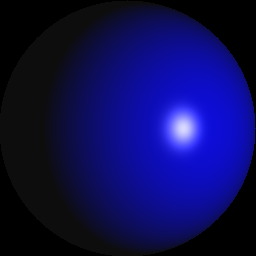
\includegraphics[width=0.4\linewidth]{render2.png}

    -----------------------------------------------------------------------------------
\end{center}
}



\end{document}

